\documentclass[twocolumn,preprintnumbers,amsmath,amssymb,aps,prb]{revtex4}
% Note that AJP uses the same style as Phys. Rev. B (prb).

% The % character begins a comment, which continues to the end of the line.
\usepackage{amsmath}  % needed for \tfrac, \bmatrix, etc.
\usepackage{amsfonts} % needed for bold Greek, Fraktur, and blackboard bold
\usepackage{graphicx} % needed for figures

\begin{document}

% Be sure to use the \title, \author, \affiliation, and \abstract macros
% to format your title page.  Don't use lower-level macros to  manually
% adjust the fonts and centering.

\title{Molecular dynamics simulation of synchronization in driven particles}
% In a long title you can use \\ to force a line break at a certain location.

\author{Tiare Guerrero}
\email{guer9330@pacificu.edu} % optional
%\altaffiliation[permanent address: ]{101 Main Street, 
%  Anytown, USA} % optional second address
% If there were a second author at the same address, we would put another 
% \author{} statement here.  Don't combine multiple authors in a single
% \author statement.
%\affiliation{Department of Physics, Pacific University, Forest Grove, OR 97116}
% Please provide a full mailing address here.

\author{Danielle McDermott}
\email{mcdermott@pacific.edu}
\affiliation{Department of Physics, Pacific University, Forest Grove, OR 97116}

\date{\today}

\begin{abstract}
  Synchronization
  plays a key role in many physical processes.
  We discuss a 
  molecular dynamics simulation
  of a single particle
  moving through
  a viscous liquid
  driven 
  across a washboard potential energy landscape.
  Our results show many dynamical patterns
  as we alter the landscape and driving force.
  Under certain conditions,
  the particle velocity and location
  are synchronized or 
  phase-locked,
  forming closed orbits in phase space.
  Quasi-periodic motion is common, 
  where the
  dynamical center of motion shifts the
  phase space orbit.
  This synchronized motion
  is
  observed in 
  simulations and table-top experiments,
  and
  can be used to isolate
  complex natural behaviors.
   We include molecular dynamics code
  to simulate and characterize
  particle dynamics.
\end{abstract}
% AJP requires an abstract for all regular article submissions.
% Abstracts are optional for submissions to the "Notes and Discussions" section.

\maketitle % title page is now complete

\section{Introduction} 
Synchronization is a universal phenomena
in which
individual oscillators change frequency due
to external stimuli \cite{Pikovsky2003}.
The
flickering patterns of
candle flames mediated by temperature fluctuations \cite{Okamoto2016},
vibrations of singing wineglasses interacting 
through sound waves \cite{Arane2009}, 
and metronomes vibrating through a supporting platform \cite{Jia2015}
are examples of in-phase coupled oscillations. 
Biological systems benefit from cooperative
synchronization --
birds coordinate wing flaps
to optimize energy use during flight \cite{Portugal2014},
frogs alternate croaking patterns \cite{Aihara2014},
humans clap in time with music \cite{Tranchant2016}
and 
at a cellular level, 
neurons simultaneously fire in cardiac muscle \cite{MartinHall1999}
and brain tissue \cite{Singer1999}.
External forcing can cause or regulate 
synchronization -- 
an electrical pacemaker 
regulates a heart beat 
and 
a pulsed light modifies the
flashing pattern of fireflies. 

Synchronized phase-locking or mode-locking 
first appeared in the scientific literature
with 
Huygens' 1665 experiments on
motions of synchronized 
pendula in wall-mounted clocks \cite{Bennett2002}.
A locked-mode is an integer frequency ratio.
In Huygens clocks,
the pendula were observed swing at same rate
in the same direction (1:1 mode) or
opposite directions (-1:1 mode).
A 2:1 mode occurs when a simple pendulum four
times the length of another swings with twice the period.

Complex dynamics such as synchronized mode-locking
can be studied with
colloid particles in experiments or simulations.
Typical colloids are   
plastic spheres suspended in
de-ionized water or silica beads suspended in organic solvent.
Because 
colloids are large 
and move slowly, 
particle position 
can be measured in real time 
with an optical camera \cite{Pertsinidis2001}. 
Experimental measurements of 
step-by-step dynamics of 
colloids performing phase-locked motions
are useful for
understanding synchronization at a single particle level \cite{Juniper2015,Juniper2017}. 

Light is a
tool for manipulating the colloidal environment
to alter synchronization patterns.
Colloids can be trapped
with 
radiation pressure from 
a laser beam \cite{Ashkin1997}.
A colloid centered in an optical trap is 
uniformly bombarded by photons. 
Off-center colloids 
experience a net force
due to uneven photon collisions across
the particle surface.
Depending on the 
location of the particle in the trap,
the radiation pressure either moves colloids toward center 
or ejects it from the trap.
Diffraction gratings can create
more complex light environments, 
such as periodic patterns of minima
suitable for synchronization studies \cite{Grier2003}.

The model presented in this paper
resembles an overdamped driven pendulum.
A single particle oscillator
in a potential well is 
like a skateboarder in a half-pipe or
a child on a swing.
A confined oscillator may 
synchronize its location
to the periodic pattern of the external drive,
moving back and forth in time with
the beat,
or moving between substrate minima.
When 
a constant or 
dc drive is applied,
the particle velocity is modulated by 
the landscape.
Below some threshold  
the dc force is not strong enough to push the particle
across a potential maximum so the average velocity is zero,
a phenomena referred to as pinning \cite{Reichhardt2017}.
Above the pinning threshold,
a particle subject to a constant
drive force will increase its speed at a rate proportional
to the external drive.  
When the applied force varies periodically,
the ac drive can 
cause the particle to hop back and forth across
the landscape minima.
Many synchronized patterns occur
controlled by the substrate period,
leading to 
mode-locking,
where the average particle velocity
is fixed for a range of dc drive forces \cite{Reichhardt2015}.
%-------------------------------------------------------------

%paper outline
Here we perform numerical studies 
on the synchronized dynamics
of a confined particle driven over
a washboard shaped potential energy landscape.
We describe
our molecular dynamics model for a single particle in Section~\ref{sec:MD}.
The model
is easy to simulate yet relevant
to condensed matter systems.
We summarize our results 
including synchronized motion of a single confined particle
driven across a periodic landscape in 
Section~\ref{sec:results}.
We include exercises for interested students 
in Section~\ref{sec:problems}.
In Section~\ref{sec:conclusion}
we describe how our results apply 
to physical systems
such as dusty plasmas, superconducting vortices and Josephson junctions.

\section{Molecular Dynamics Simulation}
\label{sec:MD}
We use a classical model for 
studying the dynamics of $N$ interacting particles,
using the net force on each particle to calculate
its trajectory.
Particles are confined in a two-dimensional (2D) 
simulation of area $A = L \times L$ where $L=46.\bar{6} a_0$
where $a_0$ is a dimensionless unit of length.
An individual particle $i$ has
position $\vec{r}_i = x_i \hat{x} + y_i \hat{y}$
and velocity $\vec{v}_i = d\vec{r}_i/dt$.
The edges of the system are treated with
periodic boundary conditions
such that a particle leaving the edge of the system is mapped
back to a position within the simulation boundaries 
by the transformation $x_i+L \rightarrow x_i$ and $y_i+L \rightarrow y_i$.
We show a schematic of the system in Fig.~\ref{fig:1_landscape}(a).
The units of the simulated variables are summarized in Table ~\ref{tab:1}.

We confine the particles using a position dependent 
potential energy function, called a landscape or substrate.
The landscape is modulated in the y-direction
with the periodic function 
 \begin{equation}
   U(y) = U_0 \cos{(2 \pi y / \lambda)}
     \label{eq:ysubstrate}
\end{equation}
 where $\lambda=L/N_p$ with $N_p$ are the number of periods,
 and $U_0$ is an adjustable parameter
 to set the depth of the minima
 with simulation units of energy $E_0$. 
 We plot this function in 
 Fig.~\ref{fig:1_landscape}
 for $N_p = 3$. 
 In Fig.~\ref{fig:1_landscape}(a) we show 
 the $x-y$ plane with a contour plot of $U(y)$ 
 to illustrate
 the 2D potential energy landscape,
 where 
 the maxima are colored red and the minima colored blue.
 The confining force on a particle $i$
 is calculated as 
 $\vec{F}^{l}_i(\vec{r}_i) = -\nabla U_l(\vec{r}_i)$.
 In Fig.~\ref{fig:1_landscape}(b) we plot the function
 $U(y)$ to illustrate how the magnitude
 $\vec{F}^{l}_i$ is calculated from particle position $y_i$.  
 
 Particles are subject an external time-dependent driving force
$\vec{F}^{d}(t)$
applied parallel to the y-direction.
We model this force as
\begin{equation}
  \vec{F}^{d}(t) = [F^{dc} + F^{ac} \sin(\omega t)] \hat{y},
    \label{eq:drive}
\end{equation}
with 
a constant component $F^{dc}$,
a time dependent component with amplitude $F^{ac}$
and frequency $\omega = 2 \pi f$.
%-----------------------------------------------------------
%overdamped model
%-----------------------------------------------------------
The inertia of 
small particles is reduced by interactions
with fluid particles \cite{Purcell1977}.
We assume 
colloids are
overdamped
so the particles do not accelerate,
i.e. suspended in a continuous viscous fluid
that dissipates energy supplied externally. 
Newton's second law for an individual particle
is simplified
by the assumption $\vec{a}_i$ is zero. 
The overdamped equation of motion for
the velocity $\vec{v}_i$ of 
an isolated particle is
\begin{equation}
  \eta \vec{v}_i = \vec{F}^l_{i}(\vec{r}_i) + \vec{F}^{d}(t).
    \label{eq:motion}
\end{equation}
with friction coefficient $\eta = 1$ in units of $v_0 / F_0$. 
The term $-\eta \vec{v}_i$
is a drag force used model 
energy dissipation from the fluid. 
We discuss friction models for
spheres moving through fluids in 
Exercise~\ref{ex:reynolds}. 

The equation of motion provides a direct calculation of the velocity
of an individual particle from location $\vec{r}_i$ 
and the simulation time.
The molecular dynamics simulation is controlled by a $for()$ loop
which runs to a maximum integer time step.
At each time step
we evaluate the net force on each particle as a function of its position
$\vec{r}_i(t)$
and then integrate
the equation of motion to move particles
to an updated position.
Since the acceleration as zero,
the integration of the equation of motion
is performed via 
the Euler method 
\begin{equation}
  \vec{r}_i(t+\Delta t) = \vec{v}_i(t) \Delta t + \vec{r}_i(t)
    \label{eq:euler}
\end{equation}
for a time step $\Delta t = 0.1 \tau$.
In 
Exercise~\ref{ex:euler}
we describe 
the numerical methods for 
solving differential equations.
%------------------------------------------------------------------
\begin{figure} % [h!]
\centering
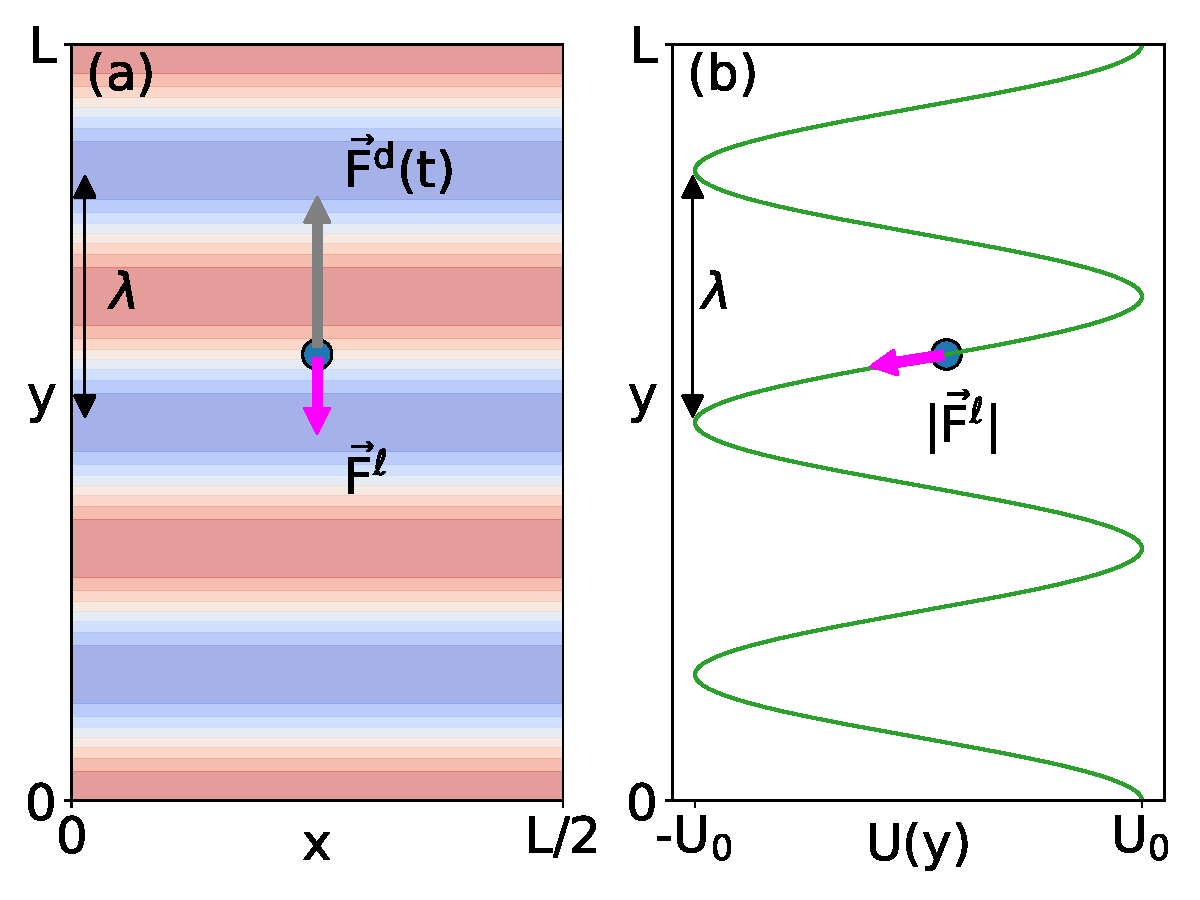
\includegraphics[width=\columnwidth]{fig1_landscape.pdf}
\caption{
  Schematic of the simulation of a single particle
  driven across a washboard potential energy landscape.
  (a) View of the $x-y$ plane. 
  The time-dependent applied driving force $\vec{F}^d$
  is parallel to the y-axis.
  The landscape is shown with 
  maxima in the potential energy marked in red
  and minima marked in blue.
  A particle is 
  subject to competing forces of the landscape and applied driving force.
  (b) The potential energy function
  along the y-axis $U_l(y)$.  
  The particle in (a) is shown at the same $y-$position.
  The slope of $U_l(y)$ is the 
  magnitude of force $\vec{F}^l$. 
  }
\label{fig:1_landscape}
\end{figure}
%
\section{Mode-locking of a single particle}
% In subsection headings, only the first word is capitalized.
\label{sec:results}
Here we drive 
a single particle 
across the landscape. 
The numerical implementation of the landscape 
is calculated with Eq.~\ref{eq:ysubstrate} as 
\begin{equation}
  \label{eq:force}
  F^l_y(y) = -A_{p} \sin{(2 \pi y / \lambda)} 
\end{equation}
where the force is scaled with parameter $A_{p} = 2\pi U_0/\lambda$.
In this section we fix the landscape parameters
to $A_{p} = 0.1 F_0$ 
with $N_p=20$ minima 
corresponding to a spatial period $\lambda = 2.3 a_0$.
The competition between the driving force and landscape potential
can produce a variety of hopping patterns in the particle motion. 
The relative values of $F^{ac}$, $F^{dc}$ and $A_p$
control the rate and distance a  particle moves 
forward and backward in the landscape.
When $F^d(t) > A_p$, a particle can 
overcome the barrier height of the landscape,
and 
the particle hops between minima in the energy landscape.
When the driving frequency is low,
as in Fig.~\ref{fig:2_Fd_vy_time},  
the driven particle 
moves 
in a pattern 
with the same frequency 
as the time-dependent force $F^d(t)$,
yet is modulated by the landscape period.
We explore changes in frequency and $F^{ac}$ 
in Ex.~\ref{ex:parameters}.
Here we vary $F^{dc}$ 
while holding the remaining parameters fixed.
%------------------------------------------------------------------------
\begin{table} %[h!]
\centering
\caption{Simulation parameters and units with comparable
  experimental values~\cite{Juniper2015,Juniper2017}.}
\begin{ruledtabular}
\begin{tabular}{c c c } 
Quantity & Simulation Unit & Experimental value\\
\hline
length &  $a_0 = 1$ & $ a_0 \sim 1.5 \mu m$\\
energy & $E_0 = 1$ & \\ %$ < E_0 <$ \\
%electric potential & $V(r_{ij}) = E_0/r_{ij}$ \\
%energy & $E_0 = q^2{Z^*}^2/4\pi \epsilon \epsilon_0 a_0$ \\
%dimensionless interaction strength & $q$ \\
%effective colloidal charge & $Z^*$ \\
%solvent dielectric constant & $\epsilon \epsilon_0$\\
force & $F_0 = E_0 / a_0$ & \\ %$<F_0<$\\
time &  $ \tau = \eta a_0 / F_0 $ & $ \tau \sim 3 sec$\\
velocity &  $ a_0 / \tau $ &  $v \sim 5 \mu m/s $\\
%driving period & $T = 100 \tau$ & $T \sim 1.3$ s \\ %frequency 0.75 Hz
%juniper uses water–ethanol mixture
substrate period & $\lambda = 2.3 a_0$ & $\lambda = 3.5 \mu m$ \\
substrate amplitude\footnote{Our substrate is scaled by our force units, while an experimental landscape is scaled by the Brownian motion of particles.} & $A_p = 0.1 F_0$ & $U_0 = 25 k_B T \sim 1 J$ \\ %$U_0 = 0.037 E_0$ 
temperature\footnote{To learn more about the effects
  of temperature on this simulation see Ex.~\ref{ex:brownian} where we study 
  $U_0 \sim k_B T$.} & $T_0 = 0$  & $T \sim 290K $ \\
\end{tabular}
\end{ruledtabular}
\label{tab:1}
\end{table}

In Fig.~\ref{fig:2_Fd_vy_time}(a)
we plot $F^d(t)$ 
as a function of time with
constants $F^{dc}=0.07$, 
$F^{ac}=0.07$ and $f=0.01$ cycles per time unit $\tau$.
The temporal period of the driving force is
$T = 1/f = 100 \tau$ and 
the simulation has a maximum
time of $400 \tau$.
In Fig.~\ref{fig:2_Fd_vy_time}(b) 
we show the $y-$position of the particle
as a function of time,
where we 
normalize $y$ by $\lambda$.
The initial particle position is $y = 0 $. 
The particle moves
in the positive y-direction
through $\Delta y = \lambda$ over time $T$,
with 
the average velocity 
$\langle {v}_y \rangle = \lambda f$. 
The inset of Fig.~\ref{fig:2_Fd_vy_time}(b)
shows $y$ 
over one period $100\tau < t < 200 \tau$
with 
the contour plot described
in Fig.~\ref{fig:1_landscape}(a).
The motion is synchronized so the 
driving force is maximum when the landscape 
force is minimum,
as shown by the coincidence of the
steep slope in 
$y/\lambda$ 
and maxima in $F^d(t)$.
When $F^d(t)$ is large 
the particle moves across the substrate minima,
shown in blue with the contour plot.
The slope of $y/\lambda$ is zero twice
during a driving period,
indicating zero
forward motion 
due to a coincidence of negative
driving force and motion over the landscape maxima.
%------------------------------------------------------------------------
\begin{figure} %[h!]
\centering
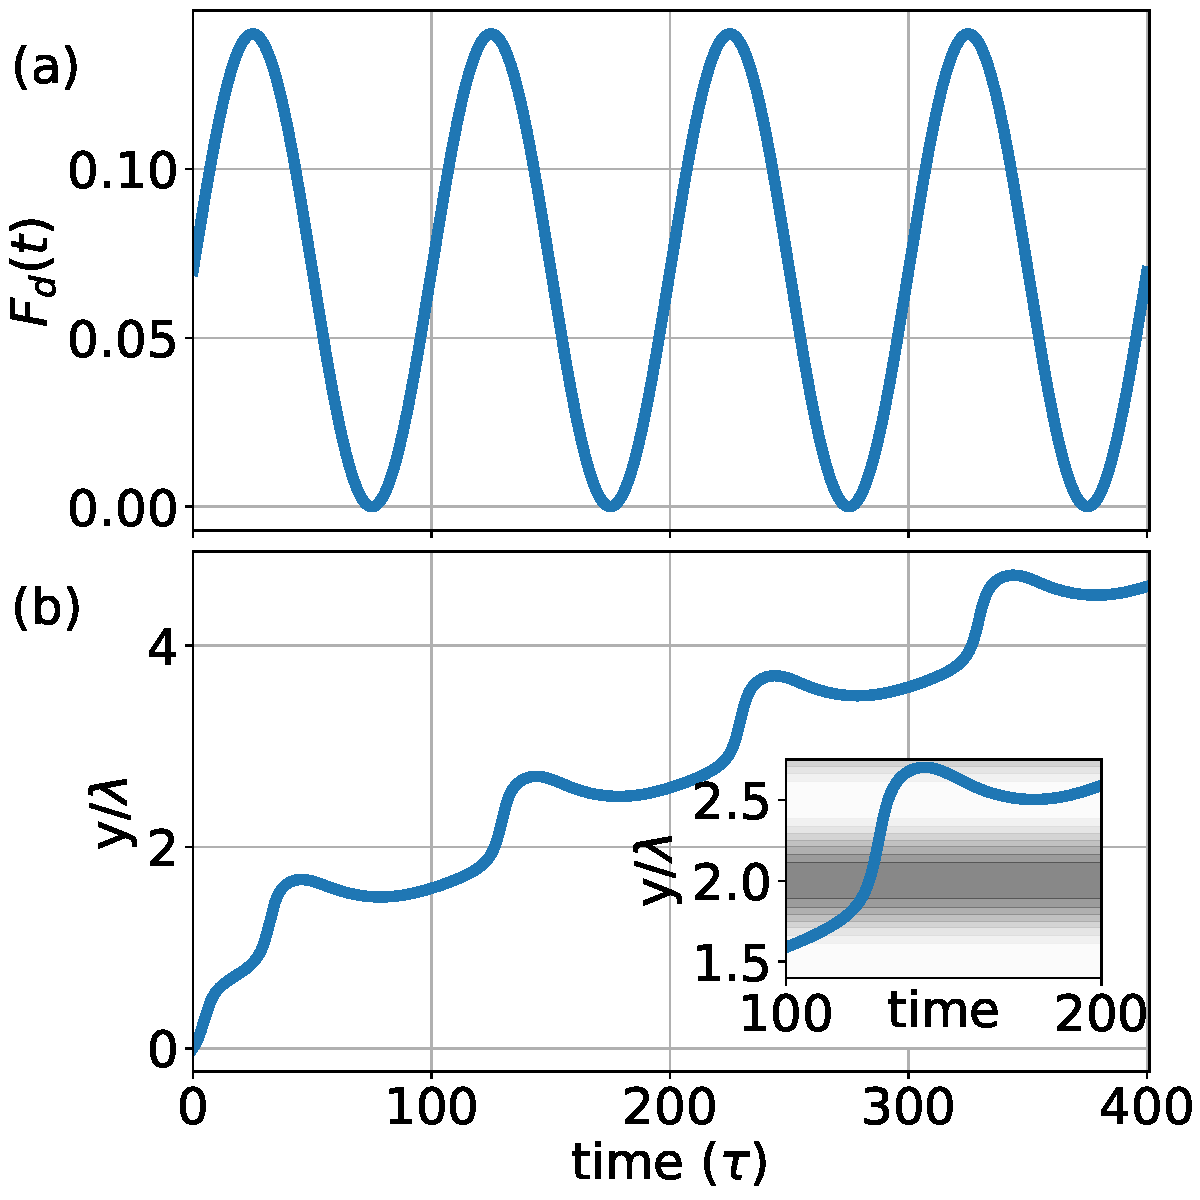
\includegraphics[width=\columnwidth]{fig2_Fd_vy_time.pdf}
\caption{(a) The applied driving force $F^d(t)$ 
  with parameters $F^{dc} = 0.07$, $F^{dc} = 0.07$ and $f=0.01$.
  (b) 
  The $y-$position of the driven particle
  normalized by the period of the substrate $\lambda$.
  The substrate strength is $A_p=0.1$.
  The inset of (b) shows
  the $y-$position
  through the second period $100\tau<t<200\tau$
  against the contour plot depicting
  the landscape potential described in Fig.~\ref{fig:1_landscape}(a).
  }
\label{fig:2_Fd_vy_time}
\end{figure}

To explore the possible hopping patterns,
we sweep through a range of $F^{dc}$ for fixed $F^{ac}$ and $A_p$.
In Fig.~\ref{fig:3_sweep_vyFDC} 
we increase $F^{dc}$ in increments of $0.001 F_0$
and 
measure the average velocity $\langle v_y \rangle $ 
as a function of $F^{dc}$.
We also perform the sweep for a non-oscillatory drive $F^{ac} = 0.0$.
With no oscillating component of the driving force,
  the force-velocity relationship is monotonically increasing
  above the depinning threshold $F^c$ such that
  \begin{equation}
    \langle v_y \rangle \propto (F^{dc}-F^c)^{-\beta}.
  \end{equation}
  The critical force $F^c$ is equal to the maximum substrate force
  $A_p$. 
  The addition of an $ac$ drive leads
  to the formation of modes.
  A mode is a periodic pattern of hops
  with a constant average particle velocity, $\langle {v}_{y} \rangle$
  over a range of driving forces $F^{dc}$.
  In Fig.~\ref{fig:3_sweep_vyFDC}
  we sweep $F^{dc}$
  with $F^{ac} = 0.07$ and $f=0.01$.
Each step represents a different pattern of hops
between substrate minima
performed by the particle
due to the landscape confinement.  
At 
low $F^{dc}$ the average velocity $\langle v_y \rangle$ is zero.
Since 
$A_p$ is large compared to the extrema of $F^{d}(t)$,
the particle oscillates back and forth
in a single minima with no net velocity,
a 0:0 mode.
At higher $F^{dc}$ the particle velocity 
$\langle v_{y} \rangle$ increases in steps of uniform height,
$\langle v_{y} \rangle = n \lambda f$,
where $n$ is an integer.
Here we observe a mode of $n=1$
for the range $0.05 < F^{dc} < 0.08$,
$n=2$ for $0.08 < F^{dc} < 0.11$,
$n=3$ for $0.12 < F^{dc} < 0.13$,
$n=4$ for $0.14 < F^{dc} < 0.155$ and 
$n=5$ for $0.155 < F^{dc} < 0.16$.
Higher modes are not visible.
The step width is non-linear
and depends on the strength of $F^{ac}$
as a Bessel function 
for this landscape potential \cite{Reichhardt2000,Juniper2017}.
Known at Shapiro steps,
these can have a variety of
interesting patterns
such as a devil's staircase related to chaotic dynamics \cite{Bak1986}.
\begin{figure} %[h!]
\centering
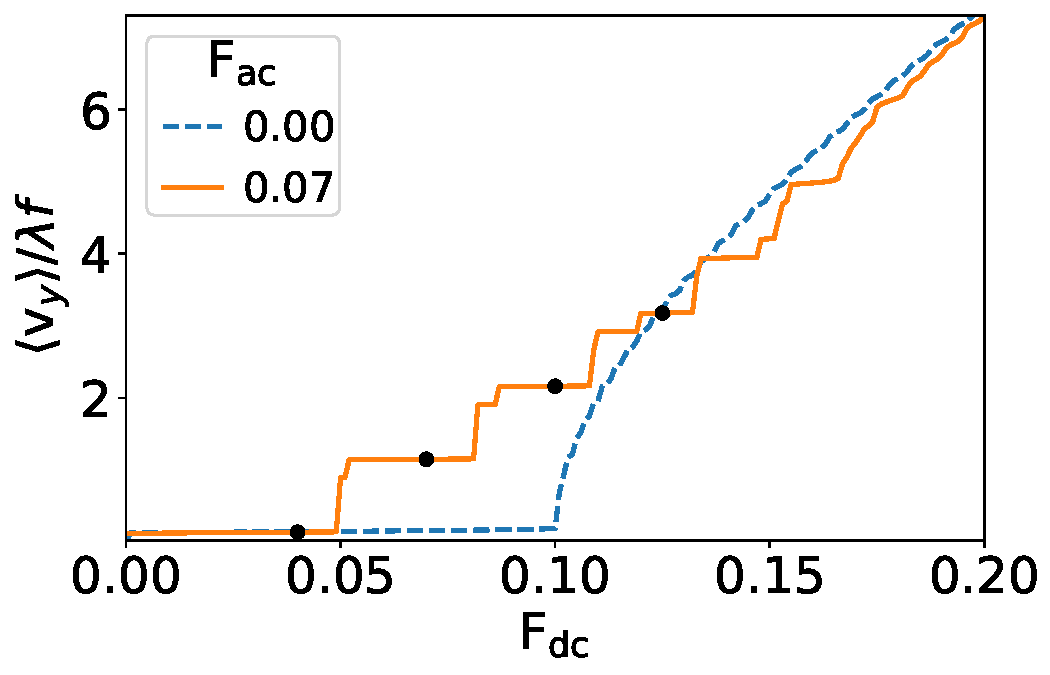
\includegraphics[width=\columnwidth]{fig3_sweep_vyFDC.pdf}
\caption{Average particle velocity  $\langle v_{y} \rangle$
  as a function of $F^{dc}$, 
  the constant parameter of $F^d(t)$ defined in Eq.~\ref{eq:drive}.
  We fix
  $F^{ac}=0.0$ (blue) and 
  $F^{ac}=0.07$ (orange) with $f = 0.01$ 
  as in Fig.~\ref{fig:2_Fd_vy_time}.
  Each of the first four steps
  has a marked value of $F^{dc}$,
  indicating a system
  plotted in Fig.~\ref{fig:4_phase}.
}
\label{fig:3_sweep_vyFDC}
\end{figure}

  To study synchronization patterns, 
  it is useful to compare
  mode-locked quantities 
  in a two dimensional phase plot. 
  In a driven pendulum confined to a single potential well,
  an appropriate
  phase space is particle velocity $v_y$ versus position $y$.  
  For a particle driven 
  through multiple identical wells 
  we define phase variables 
  to account for the net increase in position.
  The phase position is
  \begin{equation}
    \phi(t) = 2\pi (y(t)-\langle v_y \rangle t)/\lambda
  \end{equation}
  centered about the average particle displacement $\langle v_y \rangle t$
  and normalized by the substrate period $\lambda$ \cite{Juniper2015}.
  The phase velocity is
  \begin{equation}
    \dot{\phi}(t) =2\pi (v_y(t)-\langle v_y \rangle) /\lambda.  
  \end{equation}
  With no landscape force, 
  the phase velocity will be zero when $F^d(t) = F^{dc}$.
  When velocity
  is mode-locked to 
  a spatial location
  a closed loop appears in  
  phase space. 
  A 1:1 mode appears as a circle or oval. 
  Nodes appear 
  for higher modes,
  sometimes forming figure-eights
  or other recognizable patterns.
  A system that is nearly phase locked
  will appear as an unclosed loop.
  Such quasiperiodic systems are
  not fully synchronized
  so the position-velocity relationship
  shifts in time.
  In Fig.~\ref{fig:4_phase}, 
  all cases exhibit some phase shift 
  indicating the particle location and velocity
  are not fully synchronized.
  
  In Fig.~\ref{fig:4_phase}
  we plot $\dot{\phi}(t)$ versus $\phi(t)$
  for increasing 
  $F^{dc}$, 
  with the remaining parameters fixed as in Fig.~\ref{fig:2_Fd_vy_time}.
  For clarity our plots are normalized by the prefactor $2\pi$. 
  In Fig.~\ref{fig:4_phase}(a) with
  $F^{dc} = 0.04$
  the phase plot is a small asymmetric curve.
  A tail appears
  due to the initial transient
  motion of the particle.
  The particle is confined in a single
  substrate minima,
  and has no net velocity.
  The asymmetry is caused by bias induced by $F^{dc}$.
  In Fig.~\ref{fig:4_phase}(b)
  with $F^{dc} = 0.07$
  the phase loop is a symmetric triangular shape,
  indicating a 1:1 match between
  particle motion and velocity consistent with 
  Fig.~\ref{fig:2_Fd_vy_time}(a).
  As $F^{dc}$ 
  increases,
  nodes form in the phase diagram
  that occur due to repeated values
  of $\dot{\phi}$ over multiple phase positions.
  In Fig.~\ref{fig:4_phase}(c)
  with $F^{dc} = 0.1$
  two nodes form.
  The particle moves across $2\lambda$
  during one time period.
  In Fig.~\ref{fig:4_phase}(d)
  with $F^{dc} = 0.125$
  three nodes form as the particle moves across $3\lambda$.
    \begin{figure} %[h!]
      \centering
      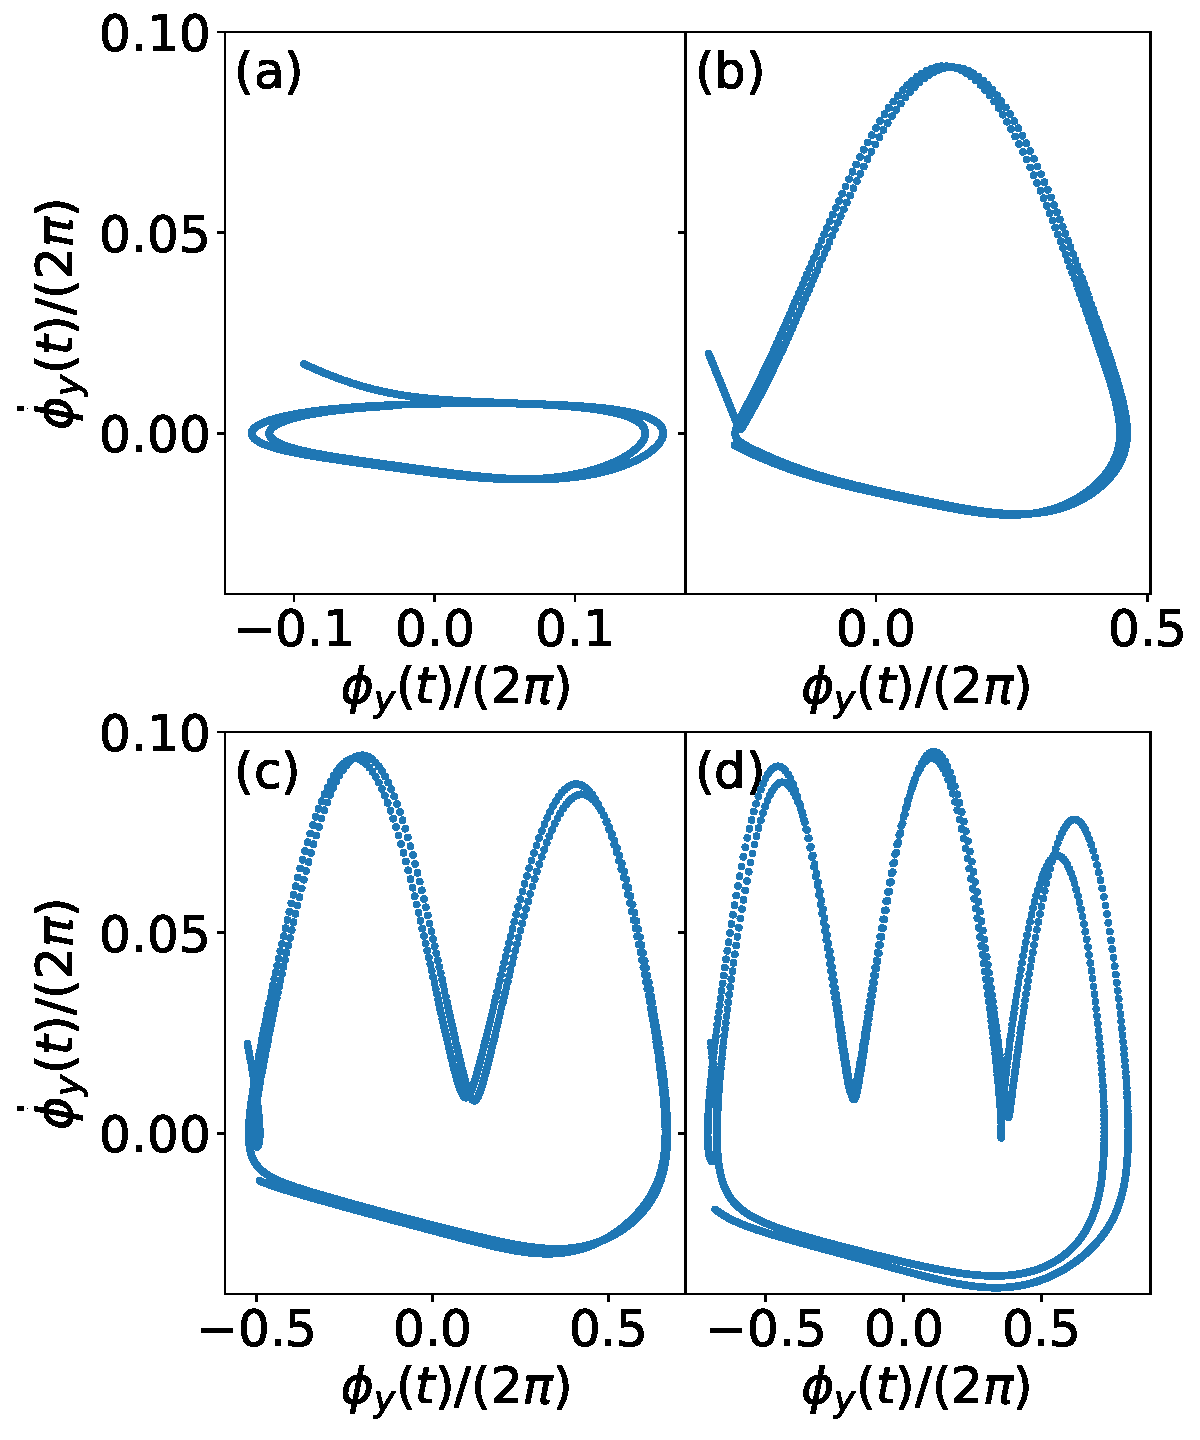
\includegraphics[width=\columnwidth]{fig4_phase.pdf}
      \caption{
        Phase plot of $\dot{\phi(t)}/(2\pi)$ vs. $\phi(t)/(2\pi)$.
        The particle is driven with $F^{dc} = $ (a) $0.04$, (b) $0.07$, (c) $0.1$, (d) $0.125$.  These values are marked as black circles
        in Fig.~\ref{fig:3_sweep_vyFDC}. 
      The other parameters
      are $F^{ac} = 0.07$, $f=0.01$, and $A_p = 0.1$
      as Fig.~\ref{fig:2_Fd_vy_time}.}
      \label{fig:4_phase}
    \end{figure}

In Section ~\ref{sec:problems}
we explore our model
with suggested exercises for interested readers.
We explore changes in the particle motion
with parameter changes in Ex.~\ref{ex:parameters}.
We include analytic exercises to examine the 
linear drag equation in Ex.~\ref{ex:reynolds}, 
the equation of motion in Ex.~\ref{ex:n2l},
and 
numerical integration techniques in Ex.~\ref{ex:euler}.
We extend the model with
numerical exercises 
to include finite temperature effects
in Ex.~\ref{ex:brownian}.

\section{Associated problems}
\label{sec:problems}	

  \subsection{Exploring model parameters}
  \label{ex:parameters}

  A range of oscillation behaviors
  can be explored by varying the
  relative strength of the confining landscape
  and external driving force.

  {\bf Explore the effect of increasing $F^{ac}$ on the hopping pattern.}
  For the single driven particle,
  the hopping patterns are typically characterized
  by $n_f$ the number of steps forward
  versus $n_b$ the number of steps backward within a single
  time period.
  The total displacement of $(n_f - n_b) \lambda$ 
  is the net hop length.  
  In Fig.~\ref{fig:2_Fd_vy_time},
  the particle moves forward through a minima ($n_f = 1$),
  and does not move backward a full minima ($n_b = 0$).  
  In order to achieve
  backwards hops,
  the driving parameters must have
  a ratio of $F^{ac}/F^{dc} > 1$ 
  and a difference $|F^{ac} - F^{dc}| > A_p$.

  In Ref.~\cite{Juniper2015}
  experiments with single colloids 
  produce 
  the following
  combinations of forward and backwards steps
  by sweeping through
  a variety of applied forces parameters $F^{dc}$ and $F^{ac}$:
  $n_f = 0$ to $6$ for $n_b = 0$,
  $n_f = 0$ to $5$ for $n_b = -1$,
  and
  $n_f = 2$ to $3$ for $n_b = -2$.
  In Fig.~\ref{fig:5_Fac_y_vs_time}
  we fix $f=0.01$, $F^{dc}=0.07$, and $A_p = 0.1$
  and increase
  the amplitude of $F^{ac}$.
  This causes the number of backwards steps to increase.
  The number of forward steps also increases
  due to the increased total positive amplitude of $F^d(t)$.
  In Fig.~\ref{fig:5_Fac_y_vs_time}(a) 
  $F^{ac} = 0.2$ %, $0.3$ and $0.4$.
  the number of backwards steps
  $n_b = 0$ with $n_f = 4$.
  In Fig.~\ref{fig:5_Fac_y_vs_time}(b) $F^{ac} = 0.4$
  $n_b = 2$ and $n_f = 6$.
  In each case the average velocity 
  is $\langle v_y \rangle = 4\lambda f$,
  which can be reproduced over a variety of $F^{ac}$ values.

  %----------------------------------------------------------
  \begin{figure} %[h!]
      \centering
      \includegraphics[width=\columnwidth]{{fig5_Fac_y_vs_time}.pdf}
      \caption{
        Motion of a particle with the same values of $F^{dc}$ and frequency as Fig.~\ref{fig:2_Fd_vy_time} and increasing $F^{ac} = $
        (a) $0.2$ and
        (b) $0.4$.
      }
      \label{fig:5_Fac_y_vs_time}
    \end{figure}
  %----------------------------------------------------------

  {\bf Explore the effect of increasing the driving frequency on the hopping pattern.}
  In Section ~\ref{sec:results}
  the frequency is sufficiently low so that 
  the applied force is large
  over a sustained time interval,
  allowing a particle to hop a substrate maxima.
  Fig.~\ref{fig:6_freq}
  shows the effects of increasing the frequency
  of applied driving force.
  We hold the remaining parameters fixed 
  to 
  $F^{dc}=0.1$, $F^{ac}=0.05$, and $A_p = 0.1$.
  We observe no backward steps 
  ($n_b = 0$) 
  across a broad range of frequencies
  since $F^{dc} - F^{ac}= 0.0$.
  The rate of forward hops 
  increases as frequency decreases,
  but in each case the particle
  hops across at most one substrate periods as in Fig.~\ref{fig:2_Fd_vy_time}.
  In Fig.~\ref{fig:6_freq}(a)
  the high frequency $f=0.05$ suppresses forward motion entirely.
  The high frequency 
  is apparent in the undulations of the particle
  with a period of $20\tau$.
    
  In Fig.~\ref{fig:6_freq}(b) the frequency $f= 0.022$
  with a period of $45\tau$
  arrests the particle between minima,
  with a hopping rate of seven periods ($320\tau$).
  At intermediate frequencies 
  such as $f=0.01$
  the particles are synchronized so that 
  the hopping rate matches the driving frequency,
  as in Fig.~\ref{fig:2_Fd_vy_time}.
  In Fig.~\ref{fig:6_freq}(c) $f=0.005$
  the particle hops forward two minima every period of $200\tau$.
  Low frequencies
  result in sustained positive motion of a particle.
  In Fig.~\ref{fig:6_freq}(e) $f=0.001$
  the hopping is continuous
  over the time $100 \tau < t < 400 \tau$,
  with the cycle repeating 
  over the period length $1000 \tau$.
  %------------------------------------------------------------
  \begin{figure} %[h!]
    \centering
    \includegraphics[width=\columnwidth]{{fig6_freq}.pdf}
    \caption{
      Motion of a particle with the same values of $F^{dc} = 0.07$ and $F^{ac} = 0.07$ as Fig.~\ref{fig:2_Fd_vy_time} and decreasing frequency $f=$ (a) $0.05$, 
        (b) $0.022$, (c) $0.005$ and (d) $0.001$. 
    }
    \label{fig:6_freq}
  \end{figure}
  %------------------------------------------------------------

  In Fig.~\ref{fig:7_sweep2_vyFDC}
  we sweep the constant driving force $F^{dc}$
  for a fixed amplitude $F^{ac}$ and frequency $f=0.01$.
  In the high frequency limit,
  the regions of phase locking
  are separated by regions of $F^{dc}$
  that do not phase lock,
  and appear to increase linearly with increasing $F^{dc}$.
  The width of the phase locked steps
  grows with increasing $F^{ac}$,
  since 
  the particle may move backwards
  over a broader range of $F^{dc}$.
  %------------------------------------------------------------
  \begin{figure} %[h!]
    \centering
    \includegraphics[width=\columnwidth]{{fig7_sweep2_vyFDC}.pdf}
      \caption{
        $\langle v_y \rangle$ vs. $F^{dc}$ of a particle with
        $F^{ac}=0.1$ (blue), $F^{ac}=0.2$ (orange),
        $F^{ac}=0.1$ (green) and $F^{ac}=0.2$ (red)
        with frequency $f=0.01$.
        The substrate is as in Fig.~\ref{fig:2_Fd_vy_time}
        with $A_p = 0.1$.
      }
      \label{fig:7_sweep2_vyFDC}
    \end{figure}
    
  \subsection{Drag models and Reynolds numbers.}
  Stokes' law describes the drag force
  $\vec{F}^{lin} = -3 \pi \eta D \vec{v}$ 
  on a sphere
  moving through a viscous liquid at velocity $\vec{v}$ 
  where $\eta$ is the dynamic fluid viscosity and 
  $D$ is the particle diameter \cite{Taylor2005}.
  In simulation we
  subsume the constants $3 \pi D$
  such that $3 \pi D \eta \rightarrow \eta $.
  Often drag forces are
  modeled as a polynomial series ~\cite{Taylor2005}
  \begin{equation}
    \vec{F}^{drag} = -b \vec{v} - c v^2 \hat{v} + \ldots  .
  \end{equation}
  Truncating the series to the first term
  is justified by demonstrating the sphere
  has a low Reynolds number  
  $R = D v \rho / \eta$
  where $\rho$ is the fluid density and $v$ the particle's speed.
  When $R$ is small, the quadratic and higher order terms
  may be ignored in favor of the linear drag term.

  To first order the viscosity is $\eta \sim 10^{-3}$ Pa-s \cite{Volpe2013}.
  {\bf Using reasonable values for the
  experimental analog of this system, 
  show that the Reynolds number is small.}
  In addition to the values listed in Table ~\ref{tab:1}, 
  the liquid density 
  $\rho \sim 10^3$ kg/cm$^3$ is a reasonable
  first order approximation
  \cite{asce}.
  
\label{ex:reynolds}

\subsection{Equation of motion}
  \label{ex:n2l}
  Newton's second law states that
  the acceleration of a particle $i$
  is proportional to 
  the sum of forces on the particle 
  \begin{equation}
  m_i \vec{a}_i = \sum \vec{F}_i
  \label{eq:n2l}
  \end{equation}
  where the constant of proportionality is the
  inertial mass $m_i$.  
  The addition of a dissipative force to a dynamical equation 
  of colloid motion 
  is typically modeled
  with a drag force proportional to the particle's velocity
  in the opposite direction of motion 
  $\vec{F}^{drag} = - \gamma \vec{v}_i$
  where $\gamma = 3 \pi \eta D$ is the drag coefficient
  described in Ex.~\ref{ex:reynolds}.
  The ratio of $m/\gamma$ is %
  known as the momentum relaxation time, %.
  and is small for
  particles with low Reynolds numbers.
  The mass of a
  typical colloid particle is $15$ picograms,
  leading to a momentum relaxation time
  on the order of microseconds.
  {\bf Confirm for the values listed in Table ~\ref{tab:1},
  the momentum relaxation time is }
  $m/\gamma \approx 0.5 ~\mu s$. 
  
  When $m/\gamma$ is small,
  particle acceleration can be ignored
  entirely.
  (a) Using Newton's Second Law for
  a small momentum relaxation time, 
  {\bf show that a particle confined to a landscape exerting force
  $F^l(\vec{r}_i)$ subject to a time dependent drive $F^d(t)$
  can be modeled with the equation of motion described in 
  Eq.~\ref{eq:motion}. }

  \subsection{Integration methods}
  \label{ex:euler}
  To calculate the position of the particle we
  integrate the equation of motion using
  the standard definition of velocity
  $\vec{v}_i = d\vec{r}_i/dt$ 
  via the 
  Euler method. 
  Our equation of motion provides
  a direct calculation for particle velocity,
  as demonstrated in Ex.~\ref{ex:n2l}.  
  When solving ordinary differential equations,
  the Euler method is effective for solving linear equations
  of the form
  $dy/dt = f(t,y(t))$ with initial condition $y(t_0) = y_0$.
  The solution is calculated algorithmically
  by stepping in time through $n$ integer steps
  $t_n = t_0 + n \Delta t$.
  At each subsequent step the new
  value for $y$ is calculated as a map solution using
  discrete times 
  $y_{n+1} = y_n + f(t_n,y_n)$.
  {\bf Apply the Euler method to our equation
  of motion to solve for the analytic expression
  of position of a particle
  $y_n$ at the $nth$ timestep (i.e. Eq.~\ref{eq:euler}).}
    
  The Euler method can be applied to
  calculate reasonable numerical solutions to 
  non-linear
  equations if the time step $\Delta t$
  is kept sufficiently small \cite{Newman}.
  In our simulations we use the timestep $\Delta t = 0.1$
  and find no change in the solution
  when we decrease the timestep to smaller values.
  In simulations
  including many interacting particles,
  a small
  timestep is essential for accurate models.
  Particle-particle interactions are typically non-linear,
  so the interparticle force changes significantly over small distances.
  Often molecular dynamics algorithms 
  are solved with higher order methods
  such as the Verlet or Runge-Kutta methods.
  These methods include  higher order terms
  that provide accurate solutions for
  second order differential equations,
  i.e. $dy/dt = v$ and $dv/dt = f_2(y,t)$.
  In Newton's second law $f_2$ would be proportional
  to the net force on a single particle.
  In our model 
  we do not integrate $f_2(y,t)$ since 
  $a = dv/dt = 0$,
  as described in Ex.~\ref{ex:n2l}.
  
  \subsection{Brownian motion}
  \label{ex:brownian}
  Brownian motion is a phenomena in which 
  visible particles change direction,
  apparently at random, 
  due to collisions with invisible fluid particles.
  The rate of collisions depends on the temperature, viscosity
  and density of 
  the suspending fluid.
  At higher temperatures
  the increased kinetic energy of particles
  makes collisions more likely, 
  as described by the Maxwell-Boltzmann distribution \cite{Einstein1905}.
  An optically trapped colloid executing Brownian motion
  is a useful probe of microscopic forces ~\cite{Volpe2013}.
  
  In molecular dynamics simulations
  it is common to treat the 
  invisible fluid particles as a continuous substance
  to reduce computational expense.
  Temperature effects
  can be modeled by applying randomized forces $f^T$
  to the visible particles.
  We use the normal distribution from the NumPy random module
  to generate a series of $f^T_n$ values for
  each integer timestep $n$ \cite{numpy}.
  A normalized random distribution of forces
  causes fluctuations in 
  motion 
  equally in all
  directions such that the force $f^T$
  averaged over a finite time interval
  is zero.  In one dimension this is expressed as 
  \begin{equation}
    \langle f^T(t) \rangle = \frac{1}{N} \sum_n^N f^T_n = 0
  \end{equation}
  where $n$ is an integer indicating
  discrete simulation timesteps and 
  $t = N \Delta t$.
  A particle
  with sufficient energy $k_b T_{min}$ may 
  hop over landscape
  barriers.
  In our simulations,
  we define temperature as 
  $k_b T/E_0 \rightarrow T$
  with constants set to unity
  to
  compare directly with force. 
 
  {\bf With no applied driving force,
    find 
    the minimum temperature required for a single particle
    to hop over maxima in the potential landscape.}
  Assume the particle is confined to
  move along the $y-$direction,
  include Brownian motion 
  in the model.
  %----------------------------------------------------
    \begin{figure} %[h!]
      \centering
      \includegraphics[width=\columnwidth]{{fig8_brownian}.pdf}
      \caption{
        Motion of a particle undergoing Brownian motion
        on a washboard potential
        energy landscape.
        (a) $T/A_p = 3.0$ no hopping occurs.
        (b) $T/A_p = 3.5$ one hop occurs and 
        (c) $T/A_p = 4.0$ many hops occur.
        Note the scale of the $y-$axis differs in each panel
        and the time scale is
        greater than in Fig.~\ref{fig:2_Fd_vy_time}.
        The precise timing of hops pattern varies
        by simulation,
        sometimes exhibiting several hops for $T/A_p = 3.5$. 
      }
      \label{fig:8_brownian}
    \end{figure}
  
  In Fig.~\ref{fig:8_brownian}
  we show the position versus time of a particle
  confined to a sinusoidal landscape
  undergoing Brownian motion.
  We increase the temperature relative
  to the amplitude of the landscape
  troughs until the particle enters a hopping regime.
  In  Fig.~\ref{fig:8_brownian}(a)
  the temperature is $T/A_p = 3.0$.
  The particle executes a 
  random walk centered at the potential minima $y/\lambda = 10$.
  We ran many simulations and never observed a hop to another minima
  within this simulation time.  
  In  Fig.~\ref{fig:8_brownian}(b)
  $T/A_p = 3.5$,  hops between
  potential minima are possible but not probable,
  a hop occurs from
  $y/\lambda = 10$ to $9$ at
  $t \sim 23000 \tau$. 
  In other simulations with identical parameters,
  we sometimes observed no hops or two hops between minima,
  as expected with random fluctuating systems.
  In  Fig.~\ref{fig:8_brownian}(c)
  $T/A_p = 4.0$ 
  we observe many hops.
  The random thermalized kicks are
  sufficiently large to make the particle perform
  what appears to be 
  a random walk of hops atop the substrate.

  For a driven particle,
  we ignore 
  the effects of temperature 
  in these simulations.  
  We note that even at $T/A_p = 4.0$ 
  the hopping rate
  is much less than the
  frequency of the applied drive.
  This can be seen in the time scale in Fig.~\ref{fig:8_brownian},
  where the average hopping rate is approximately
  every $4000\tau$,
  a value much larger than the period of the driving force.  
  At sufficiently high temperatures,
  Brownian motion does affect 
  the formation of mode-locked steps
  and can be observed in experiments.

\section{Conclusion}
\label{sec:conclusion}	
A single particle driven across a periodic potential landscape 
synchronizes its motion 
to environmental and external forces,
a phenomena known as mode-locking.  
Our simulations reproduce experiments and simulations presented in 
Juniper {\it et al.} \cite{Juniper2015, Juniper2017}
of 
mode locking in
driven colloids on a
periodic optical landscape.
Colloids are 
relatively easy to 
manipulate and image in experiments,
making ideal proxies 
for systems 
such as cold atoms or electron gases \cite{Grier2003}.
Dynamical mode-locking 
is 
observed in important technologies such as 
in quantum electronic
devices as 
stepped regions in current-voltage (I-V) relationship,
where voltage is the analog of external driving force
and current is that of particle velocity.
Known as Shapiro steps, 
these mode-locked or phase-locked currents  
have been observed due to applied ac voltages in 
single Josephson junctions \cite{Shapiro1963, Golubov2004} and
coupled arrays of junctions \cite{Benz1990}.
Shapiro steps vary in width depending on the strength of the
applied ac forces,
and are observed in a variety of ac and dc driven systems
displaying
non-Ohmic behavior in voltage-current curves,
including
charge waves, spin density waves
and superconducting vortices in landscapes 
engineered with periodic patterns of pinning sites \cite{Reichhardt2000}.
Mode-locking is a useful probe 
of complex quantum mechanical systems
since the motions of individual particles can only be inferred
from other measurements.
Our results can be relevant 
to synchronization effects
in a broad range of experiments systems
including optically confined colloids,
superconductors with periodic pinning arrays, 
and the charge and spin of atomic systems.

\begin{acknowledgments}

  We acknowledge Harvey Gould and Jan Tobochnik,
  who invited us to write the article and
  supported its development.
  Charles and Cynthia Reichhardt advised 
  the project and provided the original molecular dynamics code
  written in the C programming language.
  We acknowledge funding from the M.J. Murdock Charitable Trust
  and the Pacific Research Institute for Science and Mathematics. % (PRISM).

\end{acknowledgments}


\begin{thebibliography}{99}
% The numeral (here 99) in curly braces is nominally the number of entries in
% the bibliography. It's supposed to affect the amount of space around the
% numerical labels, so only the number of digits should matter--and even that
  % seems to make no discernible difference.
  
  %intro to oscillators
\bibitem{Pikovsky2003} A. Pikovsky, M. Rosenblum, and J. Kurths, {\it Synchronization: A Universal Concept in Nonlinear Sciences} (Cambridge Univ. Press, Cambridge, 2003).
  
\bibitem{Okamoto2016} K. Okamoto, A. Kijima, Y. Umeno, and H. Shima. Synchronization in flickering of three-coupled candle flames. Sci Rep {\bf 6}, 36145 (2016)

\bibitem{Arane2009} T. Arane, A. K. R. Musalem and M. Fridman, Coupling between two singing wineglasses, Am. J. Phys. {\bf 77}, 1066 (2009). %; https://doi.org/10.1119/1.3119175
  
\bibitem{Jia2015}  J. Jia, Z. Song, W. Liu, J. Kurths, and Xiao, J. Experimental study of the triplet synchronization of coupled nonidentical mechanical metronomes. Sci. Rep. {\bf 5}, 17008 (2015).

%Synchronization of a thermoacoustic oscillator by an external sound source
%G. Penelet and T. Biwa
%American Journal of Physics 81, 290 (2013); https://doi.org/10.1119/1.4776189
  
  %biological examples
  
\bibitem{Portugal2014} S. Portugal, T. Hubel, J. Fritz, S. Heese, D. Trobe, B. Voelkl, S. Hailes, A. M. Wilson and J. R. Usherwood.  Upwash exploitation and downwash avoidance by flap phasing in ibis formation flight. Nature {\bf 505}, 399 (2014).

  \bibitem{Aihara2014} I. Aihara, T. Mizumoto, T. Otsuka, H. Awano, K. Nagira, H. G. Okuno and K. Aihara. Spatio-Temporal Dynamics in Collective Frog Choruses Examined by Mathematical Modeling and Field Observations. Sci Rep {\bf 4}, 3891 (2014). 

  \bibitem{Tranchant2016} P. Tranchant, D. T. Vuvan, and I. Peretz, Keeping the Beat: A Large Sample Study of Bouncing and Clapping to Music. PLoS ONE 11(7): e0160178. (2016).

  \bibitem{MartinHall1999} G. Martin Hall, Sonya Bahar, and Daniel J. Gauthier, Prevalence of Rate-Dependent Behaviors in Cardiac Muscle. Phys. Rev. Lett. {\bf 82}, 2995 (1999).

    %huygens clocks
  \bibitem{Singer1999} W. Singer. Striving for coherence. Nature, {\bf 397} 391, 1999.

  \bibitem{Bennett2002} M. Bennett, M.F. Schatz, H. Rockwood, and K. Wiesenfeld, Huygens' clocks, Proc. Roy. Soc. A {\bf 458}, 563 (2002).

    
  %colloids
  \bibitem{Pertsinidis2001} A. Pertsinidis, and X. Ling,  Equilibrium Configurations and Energetics of Point Defects in Two-Dimensional Colloidal Crystals. {\it Phys Rev Lett}, {\bf 87}, 098303 (2001). %https://doi.org/10.1103/PhysRevLett.87.098303

  \bibitem{Juniper2015} M. P. N. Juniper, A. V. Straube, R. Besseling, D. G. A. L. Aarts, and R. P. A. Dullens, Microscopic dynamics of synchronization in driven colloids. Nat. Commun. 6, 7187 (2015); 
      %\bibitem{Juniper2018}
      
  \bibitem{Juniper2017} M. P. N. Juniper,  U. Zimmermann, A. V. Straube, R. Besseling, D. G. A. L. Aarts, H. L{\"o}wen, and R. P. A. Dullens,  Dynamic mode locking in a driven colloidal system: Experiments and theory. New Journal of Physics, 19(1). (2017).  %https://doi.org/10.1088/1367-2630/aa53cd

  \bibitem{Ashkin1997} A. Ashkin, Optical trapping and manipulation of neutral particles using lasers, Proc. Natl. Acad. Sci. U.S.A. 94, 4853–4860 (1997).

  \bibitem{Grier2003} D. G. Grier, A revolution in optical manipulation. Nature {\bf 424}, 810 (2003).

  %general particle on washboard
  \bibitem{Reichhardt2017} C. Reichhardt and C. J. Olson Reichhardt, “Depinning and nonequilibrium dynamic phases of particle assemblies driven over random and ordered substrates: a review,” Rep. Prog. Phys. 80, 026501 (2017).

  \bibitem{Reichhardt2015} C. Reichhardt, and C. J. O. Reichhardt,  Shapiro steps for skyrmion motion on a washboard potential with longitudinal and transverse ac drives. Phys. Rev. B {\bf 92}, (22). (2015).      

  %overdamped justification
  \bibitem{Purcell1977} E. M. Purcell, Life at low Reynolds numbers, Am. J. Phys. {\bf 45}, 3–11 (1977).
  
  %chaos!
  \bibitem{Bak1986} P. Bak. The Devil's Staircase. Physics Today {\bf 39}, 12, 38 (1986).

  %overdamped justification
  \bibitem{Taylor2005} J. Taylor,  Classical mechanics. University Science Books (2005).

  %brownian motion!
  \bibitem{Volpe2013} G. Volpe and G. Volpe, Simulation of a Brownian particle in an optical trap, Am. J. Phys. 81 (3), March 2013

  %viscosity and density citation
  \bibitem{asce}
    %Non-fundamental constants for water viscosity are available
    %in several databases including 
    %  (1) https://ascelibrary.org/doi/pdf/10.1061/9780784408230.ap02
    IAPWS R12-08, 
    Release on the IAPWS Formulation 2008 for the Viscosity of Ordinary Water Substance,  September 2008.
    %IAPWS 2008 -
    \url{http://www.iapws.org/relguide/viscosity.html}
    %[citation for these values better than wikipedia] \cite{} %CONFIRM!
    %density $\rho = 0.9982 g/cm^3$

  %numerical solutions of differential equations
  \bibitem{Newman} M. Newman, Computational Physics, CreateSpace Independent Publishing Platform. (2012).
      
    %Brownian motion!
  \bibitem{Einstein1905} A. Einstein, Investigations on the Theory of the Brownian Movement,  Dover Publications (1956).

    \bibitem{numpy} C.R. Harris, K.J. Millman, S.J. van der Walt, et al. Array programming with NumPy. Nature {\bf 585}, 357 (2020). %DOI: 0.1038/s41586-020-2649-2. (Publisher link).
      
   %Josephson Junctions and other condensed matter applications
    \bibitem{Shapiro1963} S. Shapiro, Josephson currents in superconducting tunneling: the effect of microwaves and other observations, Phys. Rev. Lett. {\bf 11}, 80 (1963).

    \bibitem{Golubov2004} A. A. Golubov, M. Yu. Kupriyanov, and E. Il{\`i}chev. The current-phase relation in Josephson junctions, Rev. Mod. Phys. {\bf 76}, 411 (2004).

    \bibitem{Benz1990}  S. P. Benz, M. S. Rzchowski, M. Tinkham, and C. J. Lobb, Fractional giant Shapiro steps and spatially correlated phase motion in 2D Josephson arrays, Phys. Rev. Lett. {\bf 64}, 693 (1990); D. Dom{\'i}nguez and J. V. Jos{\'e}, Giant Shapiro steps with screening currents, Phys. Rev. Lett. {\bf 69}, 514 (1992).

    \bibitem{Reichhardt2000} C. Reichhardt, R. T. Scalettar, G. T., Zim{\'a}nyi, N. Gr{\o}nbech-Jensen,  Phase-locking of vortex lattices interacting with periodic pinning.  Phys. Rev. B {\bf 61}, R11914 (2000).
     

\end{thebibliography}
      
\end{document}


